\begin{figure}[ht!]
    \begin{subfigure}{.5\textwidth}
    \centering
    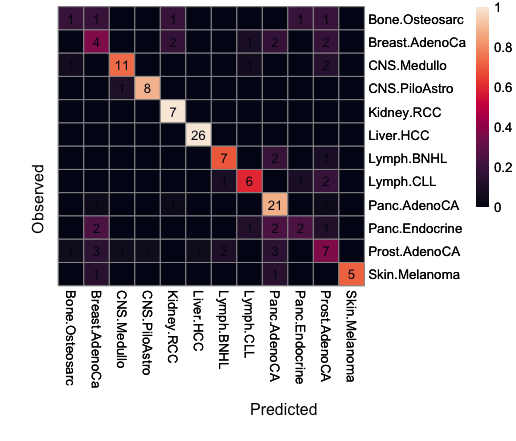
\includegraphics[width=0.9\textwidth,height=0.8\textwidth]{graphics/confusion_matrix_1mer.png}
    \caption{1-mer/asymmetry}
    \label{fig:confusion_1mer}
    \end{subfigure}
    ~
    \begin{subfigure}{.5\textwidth}
    \centering
    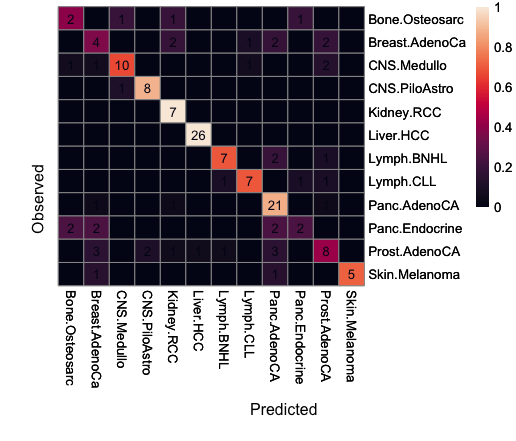
\includegraphics[width=0.9\textwidth,height=0.8\textwidth]{graphics/confusion_matrix_symmetric_1mer.png}
    \caption{1-mer/semi-symmetry}
    \label{fig:confusion_1mer_symmetric}
    \end{subfigure} \\
    \vspace{0.1cm}
    
    \begin{subfigure}{.5\textwidth}
    \centering
    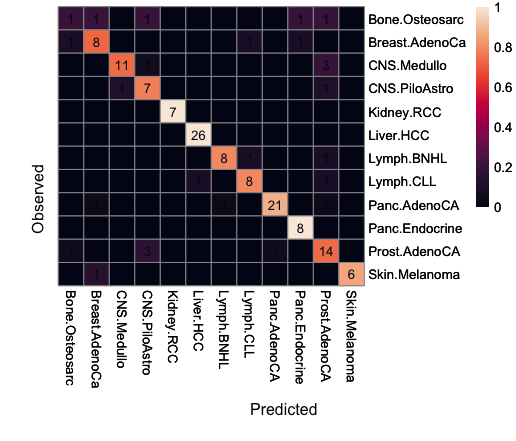
\includegraphics[width=0.9\textwidth,height=0.8\textwidth]{graphics/confusion_matrix_3mer.png}
    \caption{3-mer/asymmetry}
    \label{fig:confusion_3mer}
    \end{subfigure}
    ~
    \begin{subfigure}{.5\textwidth}
    \centering
    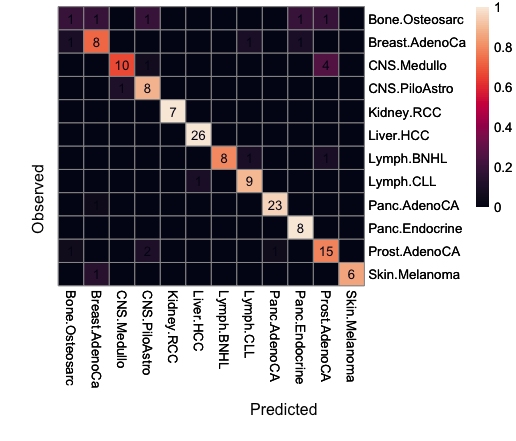
\includegraphics[width=0.9\textwidth,height=0.8\textwidth]{graphics/confusion_matrix_symmetric_3mer.png}
    \caption{3-mer/semi-symmetry}
    \label{fig:confusion_3mer_symmetric}
    \end{subfigure} \\
    \vspace{0.1cm}
    
    \begin{subfigure}{.5\textwidth}
    \centering
    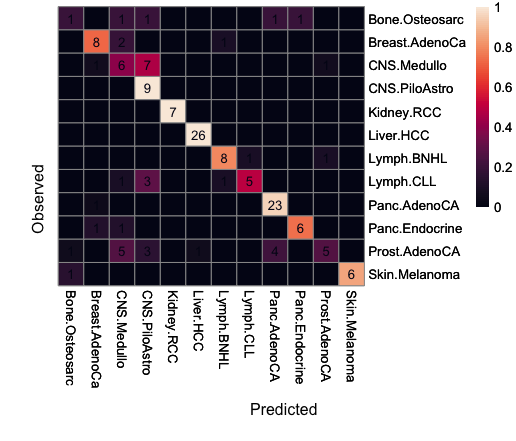
\includegraphics[width=0.9\textwidth,height=0.8\textwidth]{graphics/confusion_matrix_5mer.png}
    \caption{5-mer/asymmetry}
    \label{fig:confusion_5mer}
    \end{subfigure}
    ~
    \begin{subfigure}{.5\textwidth}
    \centering
    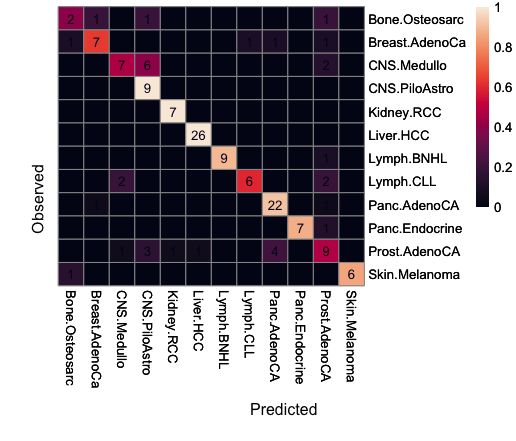
\includegraphics[width=0.9\textwidth,height=0.8\textwidth]{graphics/confusion_matrix_symmetric_5mer.png}
    \caption{5-mer/semi-symmetry}
    \label{fig:confusion_5mer_symmetric}
    \end{subfigure} \\
    
    \caption{\textbf{Representative confusion matrix, coloured by the percentage of predicted values over row total.} This is an extension of Figure \ref{fig:f1_sce}.}
    \label{fig:apdx_ml_sce}
\end{figure}